\documentclass{article}
\usepackage{tikz}

\usetikzlibrary{arrows,decorations.markings}

\title{Introduction to Political Science and American Government}
\author{Conrad A. Mearns}

\begin{document}

\maketitle

\noindent
\Large Quotes\\\\
\normalsize
\quote{A nation that hates politics will not long survive as a democracy.} - E. J. Dionne

\noindent
\Large
What is Political Science?
\normalsize

\noindent
Politics is "Who gets what, when and how?" It is the resolution of peaceful conflict or rare and scarce things.
\begin{itemize}
  \item Who --- parties, individuals, citizens, instututions
  \item What --- money, distrubution, rights, symbolism
  \item Where and How --- congressional legistlation, court, executive order, voting
\end{itemize}

\noindent
There are three kinds of statements to be made in Political Science
\begin{itemize}
  \item Descriptive --- True / False --- things that can be perceieved --- "It is snowing"
  \item Evaluative --- Good / Bad --- normative, defines morals --- "It is good that there are 100 senators"
  \item Explanatory --- Cause / Effect --- why do people vote the way they do? Ways to relate variables. --- "Trump was elected with help of foreign interference"
\end{itemize}

\noindent
It is important to differentiate cause from correlation. Post hoc ergo propter hoc --- After this, therefor because of this. It was winter, now it is spring. Therefor winter caused spring.

\noindent
Democracy can adapt. Policy that affects a majority can only be enacted with support from that majority.\\

\noindent
\Large
On Reading Sources\\
\normalsize
\noindent
Arguement - A set of proposition to lead us to a conclusion.

\begin{enumerate}
  \item Consider the source
  \item Lay out the arguement
  \item Find evidence and claims to support propositions
  \item Evaluate the conclusion
  \item Consider the consequences or purpose
\end{enumerate}

\noindent
\Large On Power and Authority\\
\normalsize
\noindent
Suppose people-entities $A$ and $B$.

\centering
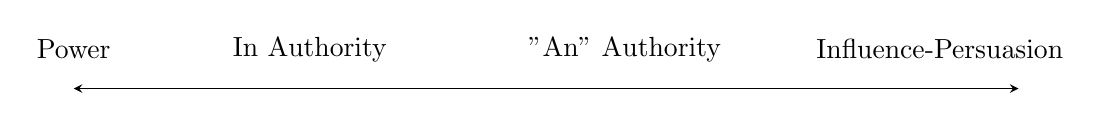
\begin{tikzpicture}
  \node (a) at (0,1) {Power};
  \node (b) at (3,1) {In Authority};
  \node (c) at (7,1) {"An" Authority};
  \node (d) at (11,1) {Influence-Persuasion};
  \draw [<->,>=stealth] (0,.5) -- (12,.5);
\end{tikzpicture}
\raggedright

\begin{itemize}
  \item Power: $A$ creates a threat to force $B$ to conform to what $A$ wants. Either by taking benifits or imposing punishment.
  \item In Authority: Power is possibly given to $A$ to threaten $B$ into doing what $A$ wants.
  \item "An" Authority: $A$ suggest $B$ to take some form of action because it benifits $B$, only because $B$ looks up to $A$.
  \item Influence-Persuassion: $A$ wants something so $A$ persuades $B$ to conform for the self interest of $B$.
\end{itemize}

\noindent
Authority is an assignment of resources of power given to a holder when needed. It does not promise control, only access or oppurtunity to power.

\noindent
\Large
On Defining Democracy\\
\normalsize
\noindent
See James Madison's Federalist Paper 10.

\indent
"Democracy" has it's roots from the Greek words d\={e}mos and -kratia, meaning "the people" and "power / rule" respectively. The democracy we know isn't the Athenian democracy originially idealized, it's actually a Republic. Athenian democracy is centered around what's popular, and participation. That is to say, Athenian democracy requires more than just voting on ideas, it requires deliberation and constant confliction. People who follow this belief are Popular Democrats.\\

Elite Democrats are the proposed solution by James Madison. He argued that humans are, by nature, private and passionate. By forming groups, we try to impose our beliefs guided by emotion and passion - self interest. Elite Democrats are to be commited to formality and compomise for the percieved greater good of everyone affected.

\noindent
\Large
On the Articles of Confederation\\
\normalsize
\indent
The Articles of Confederation gave sovereignty (supreme power and authority to govern itself) to each of the thirteen new states, with limited central control. The central government had power to "declare war, appoint military officers, sign treaties, make alliances, appoint foreign ambassadors, and manage relations with Indians." - Digital History.

This short and concise list of powers let citizen deference decrease, and led to Shae's Rebellion. The rebellion became a form of demonstration (though not intentionally) of the weaknesses each state had when government was small. It became apparent that the colonies needed to be united under a more powerful central government, which led to the current constitution.

The current constituion had some primary goals. One, limit the direct influence of the population in policy. Though undemocratic (by definition of democracy) this prevented low-information citizens from influencing policy for aything other than the public's good and wellness. Second, the central government needed a single form of currency, power to tax and coin money, and create new laws deemed necesarry and helpful.

\noindent
\Large
Creating a New Constitution\\
\normalsize
\indent

Possible ruling systems:
\begin{enumerate}
  \item Toryism\\ Also known as European Conservatism, was generally ruled as a monarchy with a strict hierarchy. Citizens were born into positions of superiority or inferiority. Superiors had an obligation to influence policy for the benift of inferiors, and inferiors had the obligation to abide.
  \item Classical Republicanism\\ Based on true democracy, Classical Republicanism required active participation in creating agreements for the public good. It relied heavily on virtuous citizens (in this cae, to be virtuous is to devote one's self to the public good. Corruption is when virtue is lost and politics is used for personal gain).This concept was pre-capitalism and anti-capitalism, as it required homogeneousness across all statuses.\\ Jefferson believed that all of the USA should be centeralized around farming, and that manufacturing should be kept in Europe. This concept would allow for homogeneous citizens and stop citizens from becoming depenedant on companies.
  \item Classical Liberalism\\ To reflect free and equal judgement to citizens. The role of government in Classical Liberalism is to do the very least to protect citizen rights. It values order with justice, economic growth and moral and scientific progress. Every citizen is absolutely free to live how they want, and to be as politically involved as they want. Because of this freedom, authority can only truely be given at the consent of the citizens, often backed with voting and law.
\end{enumerate}

\indent
Classical Liberalism is what the United States Constituion is based on. In the article, it lays the foundation for free and equal citizens to be protected by a transparent governing body. However, this system can lead to majority tyranny, as seen throughout history. Another emergence from this ideaology was capitalism, which thrives by driving citizens to work for their own self interest.


\end{document}
